\subsection{Phong shading}
Flat shading is a little brutal, especially with respect to specularity. If a
surface has large specular areas they will either be ignored, or define the
intensity of the entire surface. Phong illumination corrects this problem.

\begin{figure}[htb]
	\centering
	\scalebox{0.5}
	{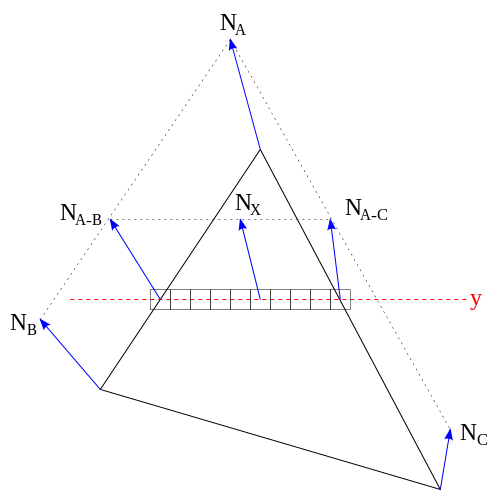
\includegraphics{pics/phongInterpol.png}}
	\caption{Normal interpolation in Phong shading}
	\label{fig:phongInterpo}
\end{figure}

By interpolating bilinearly \ref{fig:phongInterpo}

